\newpage
\part{Habitat Evaluation} \label{part:he}

\section{Introduction to Habitat Suitability evaluation} \label{sec:heintro}
The \textit{HabitatEvaluation} module creates habitat suitability index (HSI) rasters for various fish species and combines multiple HSI rasters into a composite habitat suitability index raster (cHSI or CSI). The habitat suitability index ranges between 0.0 and 1.0, according to \citet{bovee86}. It uses a threshold value for defining valuable habitat, which is initially set to 0.4; i.e., HSI values between 0.0 and 0.4 or \texttt{NoData} are considered as "non-habitat" and values between 0.4 and 1.0 correspond to valuable habitat. Currently, only hydraulic habitat suitability rasters can be calculated based on flow depth and velocity rasters for multiple discharges. A minimum of three normal discharges within the annual flow duration curve should be analyzed, e.g., the $Q_{300}$, $Q_{200}$ and $Q_{100}$, which denote the flows that are exceeded during 300, 200 and 100 days per year, respectively. The \textit{River Architect Tools} (Sec.~\ref{sec:tools}) provide the \pythoninline{make_flow_duration} routine to produce flow duration curves if required. \textit{HabitatEvaluation} uses the annual flow exceedance probabilities that are associated with the cHSI rasters for summing up the surface where the cHSI is larger than the threshold value. This surface corresponds to the Annually Usable habitat Area (AUA) in [yd$^2$ per year] or [m$^2$ per year]. The module writes relevant flows, exceedance properties and the AUA to \texttt{condition} related spreadsheets in the \texttt{HabitatEvaluation/AUA/} directory. The next sections explain the module usage:\\

\begin{tabular}{l L{0.9\textwidth}}
\multicolumn{2}{l}{}\\
Section~\ref{sec:hequick}: & Quick Guide to the application of the GUI.\\
Section~\ref{sec:heprin}:  & Working principles of the module.\\
Section~\ref{sec:hecode}:  & Descriptions of code modification possibilities.\\
\multicolumn{2}{l}{}\\
\end{tabular}



\section{Quick GUIde to habitat suitability evaluation} \label{sec:hequick}
\subsection{Main window set-up and run} 
Fig.~\ref{fig:gui_start_he} shows the \textit{HabitatEvaluation} GUI at start-up. First, the module requires a definition of relevant fish and lifestages that it reads from a workbook (see Sec.~\ref{sec:hefish}). Second, hydraulic habitat suitability rasters and related discharge exceedance probabilities need to be calculated (Sec.~\ref{sec:hemakehsi}). This last step creates habitat conditions, which can be selected in the third step. Step four combines flow depth and velocity habitat suitability rasters (Sec.~\ref{sec:herunchsi}). Step five computes the AUA (Sec.~\ref{sec:herunaua}).
 
 
\begin{figure}[hbt]
	\begin{center}
	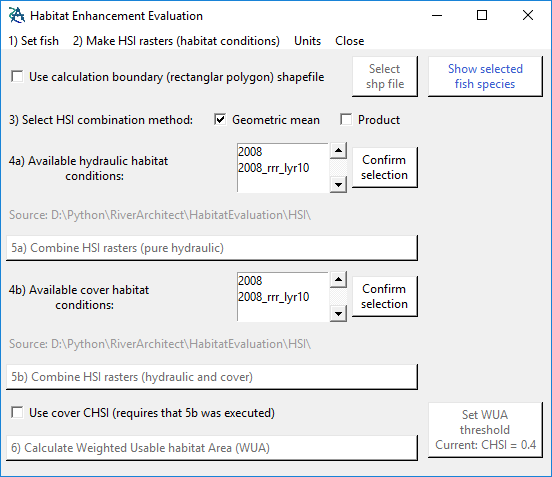
\includegraphics[width=0.7\columnwidth]{gui_start_he.PNG} % Example image
	\caption{GUI start up window. \label{fig:gui_start_he}}
	\end{center}
\end{figure}


\subsection{Input: Fish} \label{sec:hefish}
The \pythoninline{Set fish} menu enables the definition of flow depth and velocity dependent habitat suitability curves. The \pythoninline {DEFINE FISH SPECIES} menu entry opens the \texttt{Fish.xlsx} workbook, which is located in \texttt{HabitatEvaluation/.templates/}. The \texttt{Fish.xlsx} workbook contains the definition of fish species names (rows~2 to 4) and up to four lifestages per species. For every lifestage, piece-wise linear habitat suitability curves can be entered as a function of the following parameters:
\begin{itemize}
  \item Flow velocity~$u$ in row 7 to 34.
  \item Flow depth~$h$ in row 36 to 68.
  \item Substrate (grain size)~$D$ in row 70 to 77.
  \item Cover (minerals) in row 79 to 80. \texttt{Min}$\%$ describes the minimum surface occupation of either \texttt{Cobble} or \texttt{Boulder} that is required to improve habitat by a HSI value.
  \item Cover (vegetative) in row 82 to 83. \texttt{Rad.} defines the radius around single \texttt{Plants} or \texttt{Wood} placements, where habitat improves by a HSI value.
\end{itemize}

Ensure the application of the correct unit system; the drop down menu in the \texttt{Fish.xlsx} workbook automatically sets the units of flow velocity~$u$, flow depth~$h$, grain size~$D$, and delineation radius~$Rad$ around polygons. The radius~$Rad$ describes the "impact" perimeter of boulders, plants and / or wood that is drawn around the delineated polygons.

The base scenario provides habitat suitability curves for four sample fish species. More fish species can easily be appended by copy-pasting the template frame (area in thick borders in the \texttt{template} sheet) after the last defined fish species. For example, if another fish species is added to the base scenario, cells \texttt{C2} to \texttt{J83} from the \texttt{template} sheet are copied and pasted at cell \texttt{AI2} in the \texttt{fish} sheet. However, the number of lifestages per fish species and the above-stated rows need to be respected when entering piece-wise linear habitat suitability functions.\\
The structure of \texttt{Fish.xlsx} must not be modified (inserting or deleting rows or columns), unless the module's source code is also changed (not recommended). If the structure is changed anyway, the module needs to be modified as explained in Sec.~\ref{sec:hecode}.\\
Note that any relevant species-lifestage needs to have at least one entry for the velocity habitat suitability curve, as the module uses this first data cell in every column to verify if it contains data or not. For example, if a substrate habitat suitability curve is given, but the velocity habitat suitability curve is left blank, the concerned lifestage will not be considered relevant.\\

The module uses the piece-wise linear curves of habitat suitability indices to interpolate the HSI value of raster pixels. For example, if a velocity raster's pixel has a value of 0.51 (fps or m/s), the module looks up the HSI values related to the next smaller provided value (e.g., 0.5~fps or m/s) and the next higher value (e.g., 0.6~fps or m/s) and linearly interpolates the habitat suitability index for 0.51~(fps or m/s).


\subsection{Input: Combine methods (habitat suitability rasters}\label{sec:hecombine}
The module provides the options of either using the geometric mean or the product to combine depth and velocity rasters (and eventually cover rasters). The following formulae are implemented to combine a depth HSI raster~$DHSI$ with a velocity HSI raster~$VHSI$ to a $cHSI$ raster.
\begin{flalign}
  \mbox{Geometric mean:}&\mbox{\hspace{0.8cm}}&\ & cHSI =& \sqrt{DHSI \cdot VHSI} &  \mbox{\hspace{5.0cm}} &\\
  \mbox{Product:}& \mbox{\hspace{2.0cm}}&\  & cHSI =& DHSI \cdot VHSI &  \mbox{\hspace{5.0cm}} &
\end{flalign}

If a cover HSI raster~$covHSI$ is used, the following formulae apply:
\begin{flalign}
  \mbox{Geometric mean:}&\mbox{\hspace{0.8cm}}&\ & cHSI =& \sqrt[3]{DHSI \cdot VHSI \cdot covHSI} &  \mbox{\hspace{4.5cm}} & \\
  \mbox{Product:}& \mbox{\hspace{2.0cm}}&\  & cHSI =& DHSI \cdot VHSI \cdot covHSI &  \mbox{\hspace{4.5cm}} & 
\end{flalign}
The cover HSI raster~$covHSI$ represents the maximum pixel values of applied cover types (see Sec.~\ref{sec:hecombinecov} for details).

\subsection{Input: Define computation boundaries} \label{sec:hebound}
A boundary shapefile (polygon) can be selected to limit the calculation extents and assessment of the Annually Usable habitat Area AUA. Typically, that shapefile should be stored in \texttt{.../01{\myUnderscore}Conditions/\textit{condition}/boundary.shp} and it should contain one valid rectangle with an \texttt{Id} field value of \texttt{1} for that rectangle in the \texttt{Attribute table}.

\subsection{Input: HHSI} \label{sec:hemakehsi}
Before habitat suitability rasters can be calculated, at least one fish species/lifestage needs to be selected (multiple selection is possible). Then, HSI rasters can be generated by clicking on the \texttt{Generate HSI rasters} menu and \texttt{Flow depth and velocity HSI}. A new window opens and first asks for a discharge (or flow) duration curve. Clicking the associated button opens the file explorer in \texttt{HabitatEvaluation/FlowDurationCurves/}, where workbooks containing flow duration curves are located. A new flow duration curve can be generated with the \pythoninline{make_flow_duration} routine of \textit{River Architect}'s \textit{Tools} (Sec.~\ref{sec:tools}) and using \texttt{flow{\myUnderscore}duration{\myUnderscore}template.xlsx}. Any flow duration workbook needs 365 discharges (for 365 days per year) listed in column \texttt{B}, starting at row~2 in descending order. The discharges need to be positive float numbers. The associated exceedance durations (days per year) are stated in column~\texttt{C}.\\
Second, hydraulic habitat conditions need to be selected. The module looks up available hydraulic habitat conditions in \texttt{RiverArchitect/01{\myUnderscore}Conditions/}. After highlighting (click) one of the available hydraulic conditions, a click on the \texttt{Confirm selection} button generates a workbook in \texttt{RiverArchitect/Habitat Evaluation/AUA/} with the name \texttt{\textit{condition}{\myUnderscore}\textit{fil}.xlsx} for each previously selected fish. The \texttt{\textit{fil}} string abbreviates the selected fish species and lifestage, where \texttt{\textit{fi}} represents the first two letters of the fish species and \texttt{\textit{l}} the first letter of the fish lifestage. Existing workbooks for the same condition and fish are renamed (\texttt{{\myUnderscore}old} gets appended to the file name). Older \texttt{...{\myUnderscore}old.xlsx} workbooks are overwritten.\\
The generated \texttt{\textit{condition}{\myUnderscore}\textit{fil}.xlsx} can be opened by clicking on the \texttt{Optional: View discharge dependency file} button. If opened, close this workbook before continuing. Until here, only the columns \texttt{B} to \texttt{E} should contain values, which constitute the plotted flow duration curve.\\
Finally, a click on \texttt{Run (generate habitat condition)} launches the calculation of hydraulic habitat suitability index (HHSI) rasters, which are created in \texttt{RiverArchitect/HabitatEvaluation/HSI/\textit{con- dition}/}. The window starts flashing when the calculation finished. For returning to the main window (it partially freezes while the HHSI window is open), click on the \texttt{RETURN} button.

\subsection{Input: Cover HSI} \label{sec:hemakecovhsi}
As before, at least one fish species/lifestage needs to be selected (multiple selection is possible). The cover HSI raster generation can be limited to a user-defined flow region by selecting one of the \texttt{hxxx} raster names in the \pythoninline{2) Define flow region} section. However, the later combination of the cover HSI rasters with the HHSI (hydraulic HSI) rasters will automatically limit the usable habitat area to wetted pixels only. Thus, the most pertinent choice here is selecting \texttt{all terrain}. Click on \texttt{Confirm selection} to do so.\\
Relevant cover types can be selected by checking the according checkboxes, where the geofiles are required to be stored in \texttt{01{\myUnderscore}Conditions/\textit{condition}} apply the cover types:
\begin{itemize}
	\item Substrate: A \texttt{dmean} (S.I. /metric units) or \texttt{dmean{\myUnderscore}ft} (U.S. customary units) raster is required, see details in Sec.~\ref{sec:input}.
	\item Boulders: A \texttt{boulders.shp} polygon shapefile is required; the polygons delineating boulders need to have an \texttt{Short Integer}-type field called \texttt{cover} in the (\texttt{Attributes table}) and the \texttt{cover} field value of polygons is \texttt{1}.
	\item Cobbles: A \texttt{dmean} (S.I. /metric units) or \texttt{dmean{\myUnderscore}ft} (U.S. customary units) raster is required, see details in Sec.~\ref{sec:input}. Cobble is defined, where the \texttt{dmean...} raster indicates grain sizes between 0.064~m and 0.256~m.
	\item Plants: A \texttt{plants.shp} polygon shapefile is required; the polygons delineating boulders need to have an \texttt{Short Integer}-type field called \texttt{cover} in the (\texttt{Attributes table}) and the \texttt{cover} field value of polygons is \texttt{1}.
	\item Wood: A \texttt{wood.shp} polygon shapefile is required; the polygons delineating boulders need to have an \texttt{Short Integer}-type field called \texttt{cover} in the (\texttt{Attributes table}) and the \texttt{cover} field value of polygons is \texttt{1}.	
\end{itemize}

The geofiles are used with the habitat suitability (curve) definitions in the \texttt{Fish.xlsx} workbook (tab \texttt{fish}), which is located in \texttt{HabitatEvaluation/.templates/}.\\

\textit{HINT:} The applicable cover types are limited to the terms "Substrate", "Boulders", "Cobbles", "Plants", and "Wood". Bridge piers or other structural turbulence objects may constitute other cover types that are not explicitly implemented in the \textit{HabitatEvaluation} module. However, may cover types can be associated with similar effects as the implemented cover types. Thus, other cover types can be added as polygons in the shapefiles for "Boulders", "Plants", or "Wood" cover types.

\subsection{Combine habitat suitability rasters}\label{sec:herunchsi}
Back in the main window, select one available habitat condition (3) and confirm the selection. The available habitat conditions refer to the conditions created with the \texttt{Generate HSI rasters} routines (Sec.~\ref{sec:hemakehsi}). Confirming the selection activates the \texttt{Combine HSI rasters ...} buttons for launching the combination of HSI rasters. The HSI rasters can be combined either using the geometric mean or as their product by (un-)checking one of the checkboxes above the \texttt{Combine HSI rasters ...} buttons. The default combine method is \texttt{Geometric mean}. For more details, see Sec.~\ref{sec:hecombine}.\\
Two combination buttons are available: a)~\texttt{WITHOUT COVER} and b)~\texttt{WITH COVER}. Additional habitat in terms of turbulent eddies created by cobbles, boulders, submerged plants and streamwood is not well determined by 2D numerical models. \texttt{COVER} adds additional habitat as a function of the relative cobble or boulder surface and the proximity of plants or streamwood. This method values artificially placed cobbles, boulders, submerged plants and streamwood in stream restoration projects. However, the gain in AUA by using \texttt{COVER} methods is not satisfactory and the automation requires considerable efforts regarding the manual delineation of stream restoration elements. Therefore, the \texttt{WITH COVER} routines are currently only implemented as development elements without effective functionality. Currently, use the \texttt{Combine HSI rasters WITHOUT COVER} button to create cHSI rasters, which are produced in \texttt{RiverArchitect/HabitatEvaluation/CHSI/\textit{habitat{\myUnderscore}condition}/no{\myUnderscore}cover/}.

\subsection{Calculate AUA}\label{sec:herunaua}
The \texttt{Usable Area Analysis ...} buttons launch the calculation of usable habitat area based on the combined habitat suitability index (cHSI) rasters (Sec.~\ref{sec:herunchsi}). Usable (habitat) area is defined as the surface where cHSI (or CSI) pixel values are larger than the \texttt{AUA threshold}~$\theta$:
\begin{flalign}
  \mbox{AUA}&  =& \sum^{p_{Qn}}_{p_{Qi}}{\left[\sum{pixels\left(cHSI > \theta \right)}\right]\cdot p_{Qk}} &  \mbox{\hspace{8.0cm}} &
\end{flalign}

By default, this threshold value~$\theta$ is 0.4; i.e., the routine sums up the surface of pixels where the cHSI is larger than 0.4. The threshold value can be changed by clicking on the \texttt{Set AUA threshold} button. $p_{Qk}$~denotes the annual persistence of a discharge~$Q_k$ that is associated with a set of hydraulic rasters (flow depth and velocity).\\
Launch the AUA calculation by clicking on \texttt{Usable Area Analysis ...}. As before, only the \texttt{WITHOUT COVER} option effectively calculates the usable habitat area, which is saved as raster in \texttt{RiverArchitect/Habitat Evaluation/AUA/Rasters/\textit{habitat{\myUnderscore}condition}/no{\myUnderscore}cover/}. AUA is calculated in the previously created \texttt{RiverArchitect/HabitatEvaluation/AUA/\textit{condition}{\myUnderscore}\textit{fil}.xlsx} workbook (Sec. \ref{sec:hemakehsi}). The \texttt{Usable Area Analysis ...} routine fills column \texttt{F} in the workbook, which automatically calculates column \texttt{G}: AUA per discharge. The \textit{Total AUA} value in cell \texttt{J2} is the sum of column~\texttt{G}.



%----------------------------------------------------------------------------------------
\subsection{Output and application in stream restoration projects}
\label{sec:heoutput}
\subsubsection{Rasters}\label{sec:heoutputhhsi}
The module creates HHSI rasters for the selected \texttt{condition} in the folder \texttt{RiverArchitect/HabitatEvalua tion/HSI/\textit{condition}/}, where depth HSI rasters are named \texttt{dsi{\myUnderscore}\textit{fil}qqqqqq} and velocity HSI rasters are named \texttt{vsi{\myUnderscore}\textit{fil}qqqqqq}. The \texttt{qqqqqq} string refers to the discharge that is derived from the name of flow depth rasters stored in \texttt{RiverArchitect/01{\myUnderscore}Conditions/\textit{condition}/}. Please note, that the maximum discharge that can be handled is 999999~cfs or 999999~m$^3$/s because of the maximum length of raster file names.\\
CSI or cHSI rasters are created in \texttt{RiverArchitect/HabitatEvaluation/CHSI/\textit{condition}/}.\\
Rasters with relevant information for usable habitat area are created in \texttt{RiverArchitect/HabitatEvaluation/AUA/\textit{habitat{\myUnderscore}condition}/}. The raster statistics correspond to the numbers written to column \texttt{F} in \texttt{RiverArchi tect/HabitatEvaluation/AUA/\textit{condition}{\myUnderscore}\textit{fil}.xlsx}.\\


\subsubsection{Workbooks for stream restoration} \label{sec:heoutwork}
The \texttt{RiverArchitect/HabitatEvaluation/AUA/\textit{condition}{\myUnderscore}\textit{fil}.xlsx} workbook contains the key outputs of this module. The usable habitat area, related to analyzed discharges, in column~\texttt{G} and their sum (AUA) in cell~\texttt{J2} are important figures for comparing two situations (\texttt{conditions}).\\
For example, a relevant question can be "What was the annually usable habitat area for juvenile Chinook salmon in the year 2008 compared with 2014?" Comparing both the AUA in \texttt{2008{\myUnderscore}chj.xlsx} and the AUA in \texttt{2014{\myUnderscore}chj.xlsx} answers the question.\\
Another relevant question is "How much did terraforming increase AUA?". To answer this question, the habitat conditions of a (hydraulic) \texttt{condition} need to be evaluated based on 2D hydrodynamic model outputs for multiple discharges within the annual flow duration curve. Then, layer~1 features, as described in Sec.~\ref{sec:req} and the \textit{ModifyTerrain} module, need to be implemented into the DEM of the \texttt{condition}. The 2D hydrodynamic model needs to be re-run using the modified DEM and the same set of multiple annual flow duration discharges. Based on the sets of hydraulic rasters (flow depth and velocity), the \textit{HabitatEvaluation} module can compute the AUA for both conditions and selected fish species, e.g., AUA of a 2014 DEM for juvenile Chinook salmon is originally calculated in \texttt{2014{\myUnderscore}chj} and the AUA of the modified (terraformed) 2014 DEM will be contained in \texttt{2014{\myUnderscore}lyr10{\myUnderscore}chj}. Comparing the \texttt{J2} cells of both workbooks reveals the net gain in AUA. When multiple restoration variants have to be compared, the net gain in AUA of all variants can be vetted against construction costs to obtain a price in terms of US~$\$$ per yd$^2$ (or m$^2$) gain in AUA.

\subsection{Quit module and logfile}
The best option to quit the module is the \texttt{Close} dropdown menu if no background processes are going on (see terminal messages), where also the processing \texttt{habitat{\myUnderscore}evaluation.log} logfile can be opened and reviewed for any error messages. 

%----------------------------------------------------------------------------------------
\section{Working principles}\label{sec:heprin}

\subsection{Cover HSI: Substrate}\label{sec:subshsi}
A \texttt{dmean} raster is needed in the \texttt{RiverArchitect/01{\myUnderscore}Conditions/\textit{condition}/} folder. If this box is checked, a \texttt{substrate{\myUnderscore}hsi} raster is created in \texttt{RiverArchitect/HabitatEvaluation/HSI/\textit{condit ion}/}. The applied Habitat Suitability Curves can be adapted by clicking on the \texttt{Edit HSCs} button.

\subsection{Cover HSI: Boulder}\label{sec:bouhsi}
A \texttt{boulder} shapefile containing polygons with boulder sizes (diameters) needs to be available in \texttt{RiverArchite ct/HabitatEvaluation/Cover/\textit{condition}/}. The polygons need to be manually delineated for the entire region of interest. The module will convert boulder size information into a raster and retain boulders with a size larger than a threshold value. Areas, where the boulder presence covers more than 30~$\%$ of the surface get assigned an HSI value of 0.5. Both the 30~$\%$ surface ratio and the associated HSI of 0.5 can be changed for every fish species and lifestage (Sec.~\ref{sec:hefish}).

\subsection{Cover HSI: Cobble}\label{sec:cobhsi}
A \texttt{cobble} raster containing substrate sizes (cobble diameters) needs to be available in \texttt{RiverArchitect/Habi tatEvaluation/HSI/\textit{condition}/}. The module will evaluate the percentage of area that is covered with cobble larger than a threshold value (grain size). Areas, where the percentage area covers more than 30~$\%$ of the surface get assigned an HSI value of 0.3. Both the 30~$\%$ surface ratio and the associated HSI of 0.3 can be changed for every fish species and lifestage (Sec.~\ref{sec:hefish}).

\subsection{Cover HSI: Streamwood}\label{sec:woohsi}
A \texttt{streamwood} shapefile containing polygons with single wood elements needs to be available in \texttt{RiverArchitect /HabitatEvaluation/HSI/\textit{condition}/}. The module draws polygons with a user-defined radius around the streamwood polygons and assigns a value of \texttt{1} to these polygons. The new polygons are converted into a raster and an HSI value of 0.3 is assigned to \texttt{1}~pixels. The user-defined radius and the associated HSI of 0.3 can be changed for every fish species and lifestage (Sec.~\ref{sec:hefish}).

\subsection{Cover HSI: Vegetation}\label{sec:veghsi}
A \texttt{plantings} shapefile containing polygons with single plants needs to be available in \texttt{RiverArchitect/HabitatEvaluation/HSI/\textit{condition}/}. The module draws polygons with a user-defined radius around the plant polygons and assigns a value of \texttt{1} to these polygons. The new polygons are converted into a raster and an HSI value of 0.3 is assigned to \texttt{1}~pixels. The user-defined radius and the associated HSI of 0.3 can be changed for every fish species and lifestage (Sec.~\ref{sec:hefish}).


\subsection{Cover HSI combination methods}\label{sec:hecombinecov}
The cover rasters are combined by selecting the maximum value of the superposition of applied cover types: \pythoninline{covHSI = arcpy.sa.Float(arcpy.sa.CellStatistics(applied_covers, "MAXIMUM", "DATA"))}, where \pythoninline{applied_covers} is a list of \pythoninline{arcpy.Raster()} of applied cover types.


\subsection{Usable habitat area calculation}\label{sec:hewuamethods}
The usable area is measured by converting cHSI rasters to polygon shapefiles using \pythoninline{arcpy.RasterToPolygon_conversion(cHSI, polygon_shp, "NO_SIMPLIFY")}. The area of single polygons is calculated by \pythoninline{arcpy.CalculateAreas_stats(polygon_shp, self.cache + ... + "aua_eval.shp")}. The polygon areas are summed up in a loop over the polygons (\pythoninline{with arcpy.da.UpdateCursor(self.cache + ... + "aua_eval.shp", "F_AREA") as cursor: for row in cursor:}\\\pythoninline{area += float(row[0])}). The \pythoninline{area} variable contains the usable habitat area for every discharge-related cHSI raster and it is eventually written in column~\texttt{G} of \texttt{\textit{condition}{\myUnderscore}\textit{fil}.xlsx}.

\section{Code modification: Changing the structure of Fish.xlsx} \label{sec:hecode}

The \texttt{Fish.xlsx} workbook is read by the \pythoninline{Fish} class stored in \texttt{cFish.py}. The start rows for reading velocity, depth, substrate, mineral cover and vegetation cover habitat suitability curves from the workbook are hard coded in the \pythoninline{self.parameter_rows} dictionary of the \pythoninline{Fish} class. If rows were deleted or inserted, the \pythoninline{self.parameter_rows} need to be adapted.
\begin{itemize}
 \item \pythoninline{"u": row} -- \pythoninline{row} needs to correspond to the row number where the flow velocity related habitat suitability curve starts.
 \item \pythoninline{"h": row} -- \pythoninline{row} needs to correspond to the row number where the flow depth related habitat suitability curve starts.
 \item \pythoninline{"substrate": row} -- \pythoninline{row} needs to correspond to the row number where the substrate related ($D$) habitat suitability curve starts.
 \item \pythoninline{"cov_min": row} -- \pythoninline{row} needs to correspond to the row number where the mineral cover (cobbles and boulders) related habitat suitability curve starts.
 \item \pythoninline{"cov_veg": row} -- \pythoninline{row} needs to correspond to the row number where the vegetation cover (plants and wood) related habitat suitability curve starts.
\end{itemize}

The insertion or deletion of rows can be easily and robustly adapted by changing the above dictionary items.\\

However, changing or deleting columns is more complex because the module is coded in a manner that it can theoretically read an infinite number of fish species, but always limited to the same number of lifestages. Preferably omit non-relevant lifestages (do not put any number). Otherwise, change the code where read columns are relative incremental increases of numeric column values, starting at \pythoninline{self.species_row = 2}. For example, the \pythoninline{"spawning"} lifestage is at first place, and therefore, its relative column is \pythoninline{1}. The \pythoninline{"fry"} lifestage is at second place but it needs to jump over an extra \pythoninline{u} column. Therefore, the relative column of \pythoninline{"fry"} is \pythoninline{3}, the relative column of \pythoninline{"juvenile"} is \pythoninline{5} and the relative column of \pythoninline{"adult"} is \pythoninline{7}. If another lifestage is used for any fish species, it needs to match one of the before mentioned stored in the \pythoninline{self.ls_col_add} dictionary of the \pythoninline{Fish} class. For example, the base scenario uses \textit{Lamprey} fish and a \pythoninline{"ammocoetes"} lifestage instead of \pythoninline{"fry"}. Therefore, the entry \pythoninline{"ammocoetes": 3} needs to be added to \pythoninline{self.ls_col_add}.

%\begin{python}
%  if self.units == "us":
%      self.convert_volume_to_cy = 0.037 #ft3 -> cy: float((1/3)**3)
%      self.unit_info = " cubic yard"
%      self.volume_threshold = 0.99 # -- CHANGE lod US customary HERE --
%  else:
%      self.convert_volume_to_cy = 1.0
%      self.unit_info = " cubic meter"
%      self.volume_threshold = 0.30 # -- CHANGE lod SI metric HERE --
%\end{python}

